\documentclass[12pt, titlepage]{article}

\usepackage{fullpage}
\usepackage[round]{natbib}
\usepackage{multirow}
\usepackage{booktabs}
\usepackage{tabularx}
\usepackage{graphicx}
\usepackage{float}
\usepackage{soul}
\usepackage{hyperref}
\usepackage{caption}
\usepackage{xcolor}
\usepackage[normalem]{ulem} 
\hypersetup{
    colorlinks,
    citecolor=blue,
    filecolor=black,
    linkcolor=red,
    urlcolor=blue
}

%% Comments

\usepackage{color}

\newif\ifcomments\commentstrue %displays comments
%\newif\ifcomments\commentsfalse %so that comments do not display

\ifcomments
\newcommand{\authornote}[3]{\textcolor{#1}{[#3 ---#2]}}
\newcommand{\todo}[1]{\textcolor{red}{[TODO: #1]}}
\else
\newcommand{\authornote}[3]{}
\newcommand{\todo}[1]{}
\fi

\newcommand{\wss}[1]{\authornote{blue}{SS}{#1}} 
\newcommand{\plt}[1]{\authornote{magenta}{TPLT}{#1}} %For explanation of the template
\newcommand{\an}[1]{\authornote{cyan}{Author}{#1}}

%% Common Parts

\newcommand{\progname}{Software Engineering} % PUT YOUR PROGRAM NAME HERE
\newcommand{\authname}{Team 8 -- Rhythm Rangers\\
\\ Ansel Chen
\\ Muhammad Jawad
\\ Mohamad-Hassan Bahsoun
\\ Matthew Baleanu
\\ Ahmed Al-Hayali} % AUTHOR NAMES                  

\usepackage{hyperref}
    \hypersetup{colorlinks=true, linkcolor=blue, citecolor=blue, filecolor=blue,
                urlcolor=blue, unicode=false}
    \urlstyle{same}
                                


\newcounter{acnum}
\newcommand{\actheacnum}{AC\theacnum}
\newcommand{\acref}[1]{AC\ref{#1}}

\newcounter{ucnum}
\newcommand{\uctheucnum}{UC\theucnum}
\newcommand{\uref}[1]{UC\ref{#1}}

\newcounter{mnum}
\newcommand{\mthemnum}{M\themnum}
\newcommand{\mref}[1]{M\ref{#1}}

\begin{document}

\title{Module Guide for \progname{}} 
\author{\authname}
\date{\today}

\maketitle

\pagenumbering{roman}

\section{Revision History}

\begin{tabularx}{\textwidth}{p{3cm}p{2cm}X}
\toprule {\bf Date} & {\bf Version} & {\bf Notes}\\
\midrule
Date 1 & 1.0 & Notes\\
Date 2 & 1.1 & Notes\\
\bottomrule
\end{tabularx}

\newpage

\section{Reference Material}

This section records information for easy reference.

\subsection{Abbreviations and Acronyms}

\renewcommand{\arraystretch}{1.2}
\begin{tabular}{l l} 
  \toprule		
  \textbf{symbol} & \textbf{description}\\
  \midrule 
  AC & Anticipated Change\\
  DAG & Directed Acyclic Graph \\
  M & Module \\
  MG & Module Guide \\
  OS & Operating System \\
  R & Requirement\\
  SC & Scientific Computing \\
  SRS & Software Requirements Specification\\
  \progname & Music Feature Engineering \& Recommendation Program\\ % Anticipates merging of PR suggesting changing \progname from "Software Engineering" to "GenreGuru"
  UC & Unlikely Change \\
  API & Application Program Interface \\
  (G)UI & (Graphical) User Interface \\
  BPM & Beats Per Minute \\
  WAV & Waveform Audio File Format \\
  REST(ful) & REpresentational State Transfer \\
  JSON & JavaScript Object Notation \\
  ID & IDentifier \\
  \bottomrule
\end{tabular}\\

\newpage

\tableofcontents

\listoftables

\listoffigures

\newpage

\pagenumbering{arabic}

\section{Introduction}

Decomposing a system into modules is a commonly accepted approach to developing
software.  A module is a work assignment for a programmer or programming
team~\citep{ParnasEtAl1984}.  We advocate a decomposition
based on the principle of information hiding~\citep{Parnas1972a}.  This
principle supports design for change, because the ``secrets'' that each module
hides represent likely future changes.  Design for change is valuable in SC,
where modifications are frequent, especially during initial development as the
solution space is explored.  

Our design follows the rules layed out by \citet{ParnasEtAl1984}, as follows:
\begin{itemize}
\item System details that are likely to change independently should be the
  secrets of separate modules.
\item Each data structure is implemented in only one module.
\item Any other program that requires information stored in a module's data
  structures must obtain it by calling access programs belonging to that module.
\end{itemize}

After completing the first stage of the design, the Software Requirements
Specification (SRS), the Module Guide (MG) is developed~\citep{ParnasEtAl1984}. The MG
specifies the modular structure of the system and is intended to allow both
designers and maintainers to easily identify the parts of the software.  The
potential readers of this document are as follows:

\begin{itemize}
\item New project members: This document can be a guide for a new project member
  to easily understand the overall structure and quickly find the
  relevant modules they are searching for.
\item Maintainers: The hierarchical structure of the module guide improves the
  maintainers' understanding when they need to make changes to the system. It is
  important for a maintainer to update the relevant sections of the document
  after changes have been made.
\item Designers: Once the module guide has been written, it can be used to
  check for consistency, feasibility, and flexibility. Designers can verify the
  system in various ways, such as consistency among modules, feasibility of the
  decomposition, and flexibility of the design.
\end{itemize}

The rest of the document is organized as follows. Section
\ref{SecChange} lists the anticipated and unlikely changes of the software
requirements. Section \ref{SecMH} summarizes the module decomposition that
was constructed according to the likely changes. Section \ref{SecConnection}
specifies the connections between the software requirements and the
modules. Section \ref{SecMD} gives a detailed description of the
modules. Section \ref{SecTM} includes two traceability matrices. One checks
the completeness of the design against the requirements provided in the SRS. The
other shows the relation between anticipated changes and the modules. Section
\ref{SecUse} describes the use relation between modules.

\section{Anticipated and Unlikely Changes} \label{SecChange}

This section lists possible changes to the system. According to the likeliness
of the change, the possible changes are classified into two
categories. Anticipated changes are listed in Section \ref{SecAchange}, and
unlikely changes are listed in Section \ref{SecUchange}.

\subsection{Anticipated Changes} \label{SecAchange}

Anticipated changes are the source of the information that is to be hidden
inside the modules. Ideally, changing one of the anticipated changes will only
require changing the one module that hides the associated decision. The approach
adapted here is called design for
change.

\begin{description}
\item[\refstepcounter{acnum} \actheacnum \label{acHardware}:] Format and constraints of the initial input data
\item[\refstepcounter{acnum} \actheacnum \label{acInput}:] The APIs used to fetch data
\item[\refstepcounter{acnum} \actheacnum \label{acInput}:] Feature extraction algorithms
\item[\refstepcounter{acnum} \actheacnum \label{acInput}:] Song Recommendation algorithm
\item[\refstepcounter{acnum} \actheacnum \label{acInput}:] Database Strucutre and Content
\item[\refstepcounter{acnum} \actheacnum \label{acInput}:] GUI Implementation
\item[\refstepcounter{acnum} \actheacnum \label{acInput}:] Addition and/or removal of new/old features
\end{description}

% \wss{Anticipated changes relate to changes that would be made in requirements,
% design or implementation choices.  They are not related to changes that are made
% at run-time, like the values of parameters.}

\subsection{Unlikely Changes} \label{SecUchange}

The module design should be as general as possible. However, a general system is
more complex. Sometimes this complexity is not necessary. Fixing some design
decisions at the system architecture stage can simplify the software design. If
these decision should later need to be changed, then many parts of the design
will potentially need to be modified. Hence, it is not intended that these
decisions will be changed.

\begin{description}
\item[\refstepcounter{ucnum} \uctheucnum \label{ucIO}:] Source of the input is always from the user
\item[\refstepcounter{ucnum} \uctheucnum \label{ucIO}:] the usse of Spotify and Deezer as data sources
\item[\refstepcounter{ucnum} \uctheucnum \label{ucIO}:] the goal of the system is to extract features and recommend songs
\end{description}

\section{Module Hierarchy} \label{SecMH}

This section provides an overview of the module design. Modules are summarized
in a hierarchy decomposed by secrets in Table \ref{TblMH}. The modules listed
below, which are leaves in the hierarchy tree, are the modules that will
actually be implemented.

\begin{description}
\item [\refstepcounter{mnum} \mthemnum \label{mHH}:] Hardware-Hiding Module
\item ...
\end{description}


\begin{table}[h!]
\centering
\begin{tabular}{p{0.3\textwidth} p{0.6\textwidth}}
\toprule
\textbf{Level 1} & \textbf{Level 2}\\
\midrule

{Hardware-Hiding Module} & ~ \\
\midrule

\multirow{7}{0.3\textwidth}{Behaviour-Hiding Module} & ?\\
& ?\\
& ?\\
& ?\\
& ?\\
& ?\\
& ?\\ 
& ?\\
\midrule

\multirow{3}{0.3\textwidth}{Software Decision Module} & {?}\\
& ?\\
& ?\\
\bottomrule

\end{tabular}
\caption{Module Hierarchy}
\label{TblMH}
\end{table}

\section{Connection Between Requirements and Design} \label{SecConnection}

The design of the system is intended to satisfy the requirements developed in
the SRS. In this stage, the system is decomposed into modules. The connection
between requirements and modules is listed in Table~\ref{TblRT}.


% \wss{The intention of this section is to document decisions that are made
%   ``between'' the requirements and the design.  To satisfy some requirements,
%   design decisions need to be made.  Rather than make these decisions implicit,
%   they are explicitly recorded here.  For instance, if a program has security
%   requirements, a specific design decision may be made to satisfy those
%   requirements with a password.}

\section{Module Decomposition} \label{SecMD}

Modules are decomposed according to the principle of ``information hiding''
proposed by \citet{ParnasEtAl1984}. The \emph{Secrets} field in a module
decomposition is a brief statement of the design decision hidden by the
module. The \emph{Services} field specifies \emph{what} the module will do
without documenting \emph{how} to do it. For each module, a suggestion for the
implementing software is given under the \emph{Implemented By} title. If the
entry is \emph{OS}, this means that the module is provided by the operating
system or by standard programming language libraries.  \emph{\progname{}} means the
module will be implemented by the \progname{} software.

Only the leaf modules in the hierarchy have to be implemented. If a dash
(\emph{--}) is shown, this means that the module is not a leaf and will not have
to be implemented.

\begin{table}[h!]
  \centering
  \begin{tabular}{p{0.3\textwidth} p{0.6\textwidth}}
  \toprule
  \textbf{Level 1} & \textbf{Level 2}\\
  \midrule
  
  {Hardware-Hiding} & ~ \\
  \midrule
  
  \multirow{7}{0.3\textwidth}{Behaviour-Hiding} & GUI Module\\
  & Audio File Upload Module\\
  & Search Query Module\\
  & Client Communication Module\\
  %server side
  & Server Communication Module\\
  & Driver Module\\
  %feature extractions
  & Tempo (BPM) Feature Extraction Module\\
  & Key and Scale Feature Extraction Module\\
  & \textcolor{red}{\st{Instrument Type Feature Extraction Module}}\\
  & \textcolor{red}{\st{Vocal Gender Feature Extraction Module}}\\
  & \textcolor{red}{\st{Mood Feature Extraction Module}}\\
  & Dynamic Range Feature Extraction Module\\
  & \textcolor{red}{RMS feature Module}\\
  & Instrumentalness Feature Extraction Module\\
  & \textcolor{red}{\st{Contour Feature Extraction Module}}\\
  & \textcolor{red}{Spectral Centroid Feature Module}\\
  & \textcolor{red}{Spectral Bandwidth Feature Module}\\
  & \textcolor{red}{Spectral Rolloff Feature Module}\\
  & \textcolor{red}{Spectral Flux Feature Module}\\
  & \textcolor{red}{Spectral Contrast Feature Module}\\
  %final pieces
  & Recommendation Module\\
  & Program Results Interface Module\\
  \midrule
  
  \multirow{3}{0.3\textwidth}{Software Decision} & Database\\
  & Spotify API\\
  & Deezer API\\
  & \textcolor{red}{\st{Genre Feature Module}}\\
  & \textcolor{red}{Spleeter Audio Splitter Module}\\
  \bottomrule
  
  \end{tabular}
  \caption{Module Hierarchy}
  \label{TblMH}
  \end{table}

\subsection{Hardware Hiding Modules (\mref{mHH})}

\begin{description}
\item[N/A]
\end{description}

\subsection{Behaviour-Hiding Module}

\begin{description}
\item[Secrets:]The contents of the required behaviours.
\item[Services:]Includes programs that provide externally visible behaviour of
  the system as specified in the software requirements specification (SRS)
  documents. This module serves as a communication layer between the
  hardware-hiding module and the software decision module. The programs in this
  module will need to change if there are changes in the SRS.
  %services need to be reworded - check hunter's doc
  %https://github.com/cer-hunter/OAR-CAS741/blob/main/docs/Design/SoftArchitecture/MG.pdf
\item[Implemented By:] --
\end{description}

%master input - might need to break this down more? seems like GUI should actually be
%software decision. Refer to hunter's OAR for example
\subsubsection{GUI Module (\mref{m1})}

\begin{description}
\item[Secrets:] The format and structure of the input data.
\item[Services:] Handles user interaction, calling of the sub-input modules. 
\item[Implemented By:] Frontend UI development framework
\item[Type of Module:] Abstract Data Type
\end{description}

%input method 1
\subsubsection{Audio File Upload Module (\mref{m2})}

\begin{description}
\item[Secrets:] The format and structure of the input data.
\item[Services:] Takes in an audiofile and grabs metadata from the user. 
\item[Implemented By:] Frontend framework file upload widget
\item[Type of Module:] Abstract Data Type
\end{description}

%input method 2
\subsubsection{Search Query Module (\mref{m3})}

\begin{description}
\item[Secrets:] The format and structure of the input data.
\item[Services:] Takes in a user input, query searches it and then allows a user to select one of the query results. 
\item[Implemented By:] Frontend Framework text input widget
\item[Type of Module:] Abstract Data Type
\end{description}

%client-server comms
\subsubsection{Client Communication Module (\mref{m4})}

\begin{description}
\item[Secrets:] The format and structure of the input data.
\item[Services:] Takes in a user input, query searches it and then allows a user to select one of the query results. 
\item[Implemented By:] Python File
\item[Type of Module:] Abstract Data Type
\end{description}

\subsubsection{Server Communication Module (\mref{m5})}

\begin{description}
\item[Secrets:] The format and structure of the input data.
\item[Services:] Takes in a user input, query searches it and then allows a user to select one of the query results. 
\item[Implemented By:] Python File
\item[Type of Module:] Abstract Data Type
\end{description}

\subsubsection{Driver Module (\mref{m6})}

\begin{description}
\item[Secrets:] The format and structure of the input data.
\item[Services:] Takes in a user input, query searches it and then allows a user to select one of the query results. 
\item[Implemented By:] Python File
\item[Type of Module:] Abstract Data Type
\end{description}

%featurizers
%f1
\subsubsection{Tempo (BPM) Feature Extraction Module (\mref{m7})}

\begin{description}
\item[Secrets:] The algorithm for calculating the tempo of the track. 
\item[Services:] Extracts the Tempo (BPM) from the audio signal. 
\item[Implemented By:] Python Function
\item[Type of Module:] Abstract Data Type
\end{description}

%f2
\subsubsection{Key and Scale Feature Extraction Module (\mref{m8})}

\begin{description}
\item[Secrets:] The algorithm for calculating the key and scale of the track. 
\item[Services:]Extracts the \textbf{key} and \textbf{scale} from the audio signal. 
\item[Implemented By:] Python Function
\item[Type of Module:] Abstract Data Type
\end{description}

%f3
% \textcolor{red}{\sout{\subsubsection{Instrument Type Feature Extraction Module (\mref{m9})}}}
\subsubsection*{\textcolor{red}{\sout{Instrument Type Feature Extraction Module (\mref{m9})}}}

\begin{description}
\item \textcolor{red}{\sout{\textbf{Secrets:} The algorithm(s) for detecting the type(s) of instruments present within the track.}}
\item \textcolor{red}{\sout{\textbf{Services:} Detects the presence of different instrument types within the input audio signal.}}
\item \textcolor{red}{\sout{\textbf{Implemented By:} Python Function}}
\item \textcolor{red}{\sout{\textbf{Type of Module:} Abstract Data Type}}

\end{description}

%f4
% \subsubsection{Vocal Gender Feature Extraction Module (\mref{m10})}

% \begin{description}
% \item[Secrets:] The algorithm for detecting the overall vocal gender of the track. 
% \item[Services:]Extracts the overall vocal gender of the input audio signal. 
% \item[Implemented By:] Python Function
% \item[Type of Module:] Abstract Data Type
% \end{description}
\subsubsection*{\textcolor{red}{\sout{Vocal Gender Feature Extraction Module (\mref{m10})}}}

\begin{description}
\item \textcolor{red}{\sout{\textbf{Secrets:} The algorithm for detecting the overall vocal gender of the track.}}
\item \textcolor{red}{\sout{\textbf{Services:} Extracts the overall vocal gender of the input audio signal.}}
\item \textcolor{red}{\sout{\textbf{Implemented By:} Python Function}}
\item \textcolor{red}{\sout{\textbf{Type of Module:} Abstract Data Type}}
\end{description}

%f5
\subsubsection{Dynamic Range Feature Extraction Module (\mref{m11})}

\begin{description}
\item[Secrets:]The format and structure of the input data.
\item[Services:]Extracts the Dynamic Range (difference between peak and \textcolor{red}{\sout{through} median} in decibels) of the input audio signal.
\item[Implemented By:] Python Function
\item[Type of Module:] Abstract Data Type
\end{description}

\subsubsection{\textcolor{red}{RMS feature Module (\mref{m12})}}

\begin{description}
\item \textcolor{red}{\textbf{Secrets:} The algorithm for computing the RMS of the track}
\item \textcolor{red}{\textbf{Services:} Computes the RMS of the input audio signal.}
\item \textcolor{red}{\textbf{Implemented By:} Python Function}
\item \textcolor{red}{\textbf{Type of Module:} Abstract Data Type}
\end{description}

%f6
\subsubsection{Instrumentalness Feature Extraction Module (\mref{m12})}

\begin{description}
\item[Secrets:] The algorithm for detecting the instrumentalness of the track. 
\item[Services:] Detects the presence level of instrumentals from the input audio signal. 
\item[Implemented By:] Python Function
\item[Type of Module:] Abstract Data Type
\end{description}

%f7
% \subsubsection{Contour Feature Extraction Module (\mref{m13})}

% \begin{description}
% \item[Secrets:] The algorithm to detect the musical contour of the track. 
% \item[Services:] Extracts the musical contour of the input audio signal.  
% \item[Implemented By:] Python Function
% \item[Type of Module:] Abstract Data Type
% \end{description}
\subsubsection{\textcolor{red}{\sout{Contour Feature Extraction Module (\mref{m13})}}}

\begin{description}
\item \textcolor{red}{\sout{\textbf{Secrets:} The algorithm to detect the musical contour of the track.}}
\item \textcolor{red}{\sout{\textbf{Services:} Extracts the musical contour of the input audio signal.}}
\item \textcolor{red}{\sout{\textbf{Implemented By:} Python Function}}
\item \textcolor{red}{\sout{\textbf{Type of Module:} Abstract Data Type}}
\end{description}

%f8
% \subsubsection{Mood Feature Extraction Module (\mref{m14})}

% \begin{description}
% \item[Secrets:] The algorithm for detecting the mood of the track. 
% \item[Services:] Extracts the mood of the input audio signal. 
% \item[Implemented By:] Python Function
% \item[Type of Module:] Abstract Data Type
% \end{description}
\subsubsection{\textcolor{red}{\sout{Mood Feature Extraction Module (\mref{m14})}}}

\begin{description}
\item \textcolor{red}{\sout{\textbf{Secrets:} The algorithm for detecting the mood of the track.}}
\item \textcolor{red}{\sout{\textbf{Services:} Extracts the mood of the input audio signal.}}
\item \textcolor{red}{\sout{\textbf{Implemented By:} Python Function}}
\item \textcolor{red}{\sout{\textbf{Type of Module:} Abstract Data Type}}
\end{description}

%spectral features: centroid, flux, bandwidth, rolloff, contrast
\subsubsection{\textcolor{red}{Spectral centroid Feature Extraction Module (\mref{m12})}}

\begin{description}
\item \textcolor{red}{\textbf{Secrets:} The algorithm for detecting the Spectral centroid of the track.}
\item \textcolor{red}{\textbf{Services:} Computes the Spectral Centroid of the input audio signal.}
\item \textcolor{red}{\textbf{Implemented By:} Python Function}
\item \textcolor{red}{\textbf{Type of Module:} Abstract Data Type}
\end{description}

\subsubsection{\textcolor{red}{Spectral Bandwidth Feature Extraction Module (\mref{m12})}}

\begin{description}
\item \textcolor{red}{\textbf{Secrets:} The algorithm for detecting the Spectral Bandwidth of the track.}
\item \textcolor{red}{\textbf{Services:} Computes the spectral bandwidth of the input audio signal.}
\item \textcolor{red}{\textbf{Implemented By:} Python Function}
\item \textcolor{red}{\textbf{Type of Module:} Abstract Data Type}
\end{description}

\subsubsection{\textcolor{red}{Spectral Rolloff Feature Extraction Module (\mref{m12})}}

\begin{description}
\item \textcolor{red}{\textbf{Secrets:} The algorithm for detecting the Spectral Rolloff of the track.}
\item \textcolor{red}{\textbf{Services:} Computes the Spectral Rolloff of the input audio signal.}
\item \textcolor{red}{\textbf{Implemented By:} Python Function}
\item \textcolor{red}{\textbf{Type of Module:} Abstract Data Type}
\end{description}

\subsubsection{\textcolor{red}{Spectral Flux Feature Extraction Module (\mref{m12})}}

\begin{description}
\item \textcolor{red}{\textbf{Secrets:} The algorithm to compute the spectral flux of the track.}
\item \textcolor{red}{\textbf{Services:} Computes the spectral flux of the input audio signal.}
\item \textcolor{red}{\textbf{Implemented By:} Python Function}
\item \textcolor{red}{\textbf{Type of Module:} Abstract Data Type}
\end{description}

\subsubsection{\textcolor{red}{Spectral Contrast Feature Extraction Module (\mref{m12})}}

\begin{description}
\item \textcolor{red}{\textbf{Secrets:} The algorithm to compute the spectral contrast of the track.}
\item \textcolor{red}{\textbf{Services:} Computes the spectral contrast of the input audio signal.}
\item \textcolor{red}{\textbf{Implemented By:} Python Function}
\item \textcolor{red}{\textbf{Type of Module:} Abstract Data Type}
\end{description}


%recommendation
\subsubsection{Recommendation Module (\mref{m15})}

\begin{description}
\item[Secrets:] The recommendation machine learning algorithm. 
\item[Services:] Generates a list of recommended songs. 
\item[Implemented By:] \textcolor{red}{\sout{Machine Learning Algorithm}} \textcolor{red}{K-NN Algorithm}
\item[Type of Module:] \textcolor{red}{SKLearn Python Library}
\end{description}

%results GUI
\subsubsection{Program Results Interface Module (\mref{m16})}

\begin{description}
\item[Secrets:] The recommended songs widget and features display element. 
\item[Services:] Generates widget for recommended song(s) with preview snippet and UI element containting associated features for input song. 
\item[Implemented By:] Spotify API Calls, 
\item[Type of Module:] Abstract Data Type
\end{description}

\subsection{Software Decision Module}

\begin{description}
\item[Secrets:] The design decision based on mathematical theorems, physical
  facts, or programming considerations. The secrets of this module are
  \emph{not} described in the SRS.
\item[Services:] Includes data structure and algorithms used in the system that
  do not provide direct interaction with the user. 
  % Changes in these modules are more likely to be motivated by a desire to
  % improve performance than by externally imposed changes.
\item[Implemented By:] --
\end{description}

\subsubsection{Database Module (\mref{m17})}

\begin{description}
\item[Secrets:] The data contained in the tables. 
\item[Services:] Storages for generated features. 
\item[Implemented By:] Database Service
\item[Type of Module:] Abstract Data Object
\end{description}

% \subsubsection{Pre-Processing Module (\mref{m2})}

% \begin{description}
% \item[Secrets:]The format and structure of the input data.
% \item[Services:]Converts audio files and references into audio data for processing by featurizers
% \item[Implemented By:] Librosa Signal Processing Library
% \item[Type of Module:] Library
% \end{description}

\subsubsection{Spotify API (\mref{m18})}

\begin{description}
\item[Secrets:]Spotify API methods, credentials and metadata. 
\item[Services:]Song Metadata
\item[Implemented By:] Spotify
\item[Type of Module:] API Library
\end{description}

\subsubsection{Deezer API (\mref{m19})}

\begin{description}
\item[Secrets:]Deezer API methods, credentials and metadata. 
\item[Services:]Converts the input data into the data structure used by the
  input parameters module.
\item[Implemented By:] Deezer
\item[Type of Module:] API Library
\end{description}

\subsubsection{\textcolor{red}{Spleeter Vocal Audio Splitter(\mref{m12})}}

\begin{description}
\item \textcolor{red}{\textbf{Secrets:} Machine learning model, training data.}
\item \textcolor{red}{\textbf{Services:} Isolates vocal component of the song from non-vocal components.}
\item \textcolor{red}{\textbf{Implemented By:} Spleeter Library}
\item \textcolor{red}{\textbf{Type of Module:} Abstract Data Object}
\end{description}

% \subsubsection{Genre Feature Module (\mref{m20})}

% \begin{description}
% \item[Secrets:]Genre label for a song
% \item[Services:]Fetches a genre label for a required song
% \item[Implemented By:] Deezer API
% \item[Type of Module:] Abstract Data Type
% \end{description}

\subsubsection*{\textcolor{red}{\sout{Genre Feature Module (\mref{m20})}}}

\begin{description}
\item \textcolor{red}{\sout{\textbf{Secrets:} Genre label for a song}}
\item \textcolor{red}{\sout{\textbf{Services:} Fetches a genre label for a required song}}
\item \textcolor{red}{\sout{\textbf{Implemented By:} Deezer API}}
\item \textcolor{red}{\sout{\textbf{Type of Module:} Abstract Data Type}}
\end{description}

\section{Traceability Matrix} \label{SecTM}

This section shows two traceability matrices: between the modules and the
requirements and between the modules and the anticipated changes.

% the table should use mref, the requirements should be named, use something
% like fref
\begin{table}[H]
\centering
\begin{tabular}{p{0.2\textwidth} p{0.6\textwidth}}
\toprule
\textbf{Requirement} & \textbf{Modules}\\
\midrule
R1 (Input queries) & GUI Module, Search Query Module, Audio File Module \\
R2 (Display search results) & GUI Module, Results Display Module \\
R3 (Play previews) & GUI Module, Results Display Module, Spotify Module \\
R4 (Validate audio files) & Audio File Module \\
R5 (Convert audio to WAV) & Audio File Module, Featurizer Module \\
R6 (Construct Spotify query) & Search Query Module \\
R7 (Extract features) & Featurizer Module, Driver Module, Genre Feature Module \\
R8 (Support 8 features) & Featurizer Module, Genre Feature Module \\
R9 (Generate recommendations) & Recommendation Module, Driver Module \\
R10 (Transmit user input) & Client-Side Communication Module, Server-Side Communication Module \\
R11 (Receive recommendations) & Client-Side Communication Module, Server-Side Communication Module \\
\bottomrule
\end{tabular}
\caption{Trace Between Requirements and Modules}
\label{TblRT}
\end{table}

\subsection{Explanation of Traceability}

\begin{itemize}
    \item \textbf{R1 (Input queries):} Linked to the GUI Module, Search Query Module, and Audio File Module to handle user inputs efficiently.
    \item \textbf{R2 (Display search results):} Connected to the GUI Module and Results Display Module to display song information accurately.
    \item \textbf{R3 (Play previews):} Associated with the GUI Module, Results Display Module, and Spotify Module to enable audio playback.
    \item \textbf{R4 (Validate audio files):} Linked to the Audio File Module to ensure only valid files are processed.
    \item \textbf{R5 (Convert audio to WAV):} Handled by the Audio File Module and Featurizer Module to standardize inputs.
    \item \textbf{R6 (Construct Spotify query):} Involves the Search Query Module to generate and send API requests.
    \item \textbf{R7 (Extract features):} Requires the Featurizer Module, Driver Module, and Genre Feature Module to process audio files and extract features.
    \item \textbf{R8 (Support 8 features):} Ensures the Featurizer Module and Genre Feature Module handle all required features.
    \item \textbf{R9 (Generate recommendations):} Relies on the Recommendation Module and Driver Module to compute and return suggestions.
    \item \textbf{R10 (Transmit user input):} Linked to the Client-Side Communication Module and Server-Side Communication Module for transmitting data.
    \item \textbf{R11 (Receive recommendations):} Managed by the Client-Side Communication Module and Server-Side Communication Module for receiving processed results.
\end{itemize}


\begin{table}[H]
\centering
\begin{tabular}{p{0.2\textwidth} p{0.6\textwidth}}
\toprule
\textbf{AC} & \textbf{Modules}\\
\midrule
\acref{acHardware} & \mref{mHH}\\
\acref{acInput} & \mref{mInput}\\
\acref{acParams} & \mref{mParams}\\
\acref{acVerify} & \mref{mVerify}\\
\acref{acOutput} & \mref{mOutput}\\
\acref{acVerifyOut} & \mref{mVerifyOut}\\
\acref{acODEs} & \mref{mODEs}\\
\acref{acEnergy} & \mref{mEnergy}\\
\acref{acControl} & \mref{mControl}\\
\acref{acSeqDS} & \mref{mSeqDS}\\
\acref{acSolver} & \mref{mSolver}\\
\acref{acPlot} & \mref{mPlot}\\
\bottomrule
\end{tabular}
\caption{Trace Between Anticipated Changes and Modules}
\label{TblACT}
\end{table}

\section{Use Hierarchy Between Modules} \label{SecUse}

In this section, the uses hierarchy between modules is
provided. \citet{Parnas1978} said of two programs A and B that A {\em uses} B if
correct execution of B may be necessary for A to complete the task described in
its specification. That is, A {\em uses} B if there exist situations in which
the correct functioning of A depends upon the availability of a correct
implementation of B.  Figure \ref{FigUH} illustrates the use relation between
the modules. It can be seen that the graph is a directed acyclic graph
(DAG). Each level of the hierarchy offers a testable and usable subset of the
system, and modules in the higher level of the hierarchy are essentially simpler
because they use modules from the lower levels.

\wss{The uses relation is not a data flow diagram.  In the code there will often
be an import statement in module A when it directly uses module B.  Module B
provides the services that module A needs.  The code for module A needs to be
able to see these services (hence the import statement).  Since the uses
relation is transitive, there is a use relation without an import, but the
arrows in the diagram typically correspond to the presence of import statement.}

\wss{If module A uses module B, the arrow is directed from A to B.}

\begin{figure}[H]
\centering
%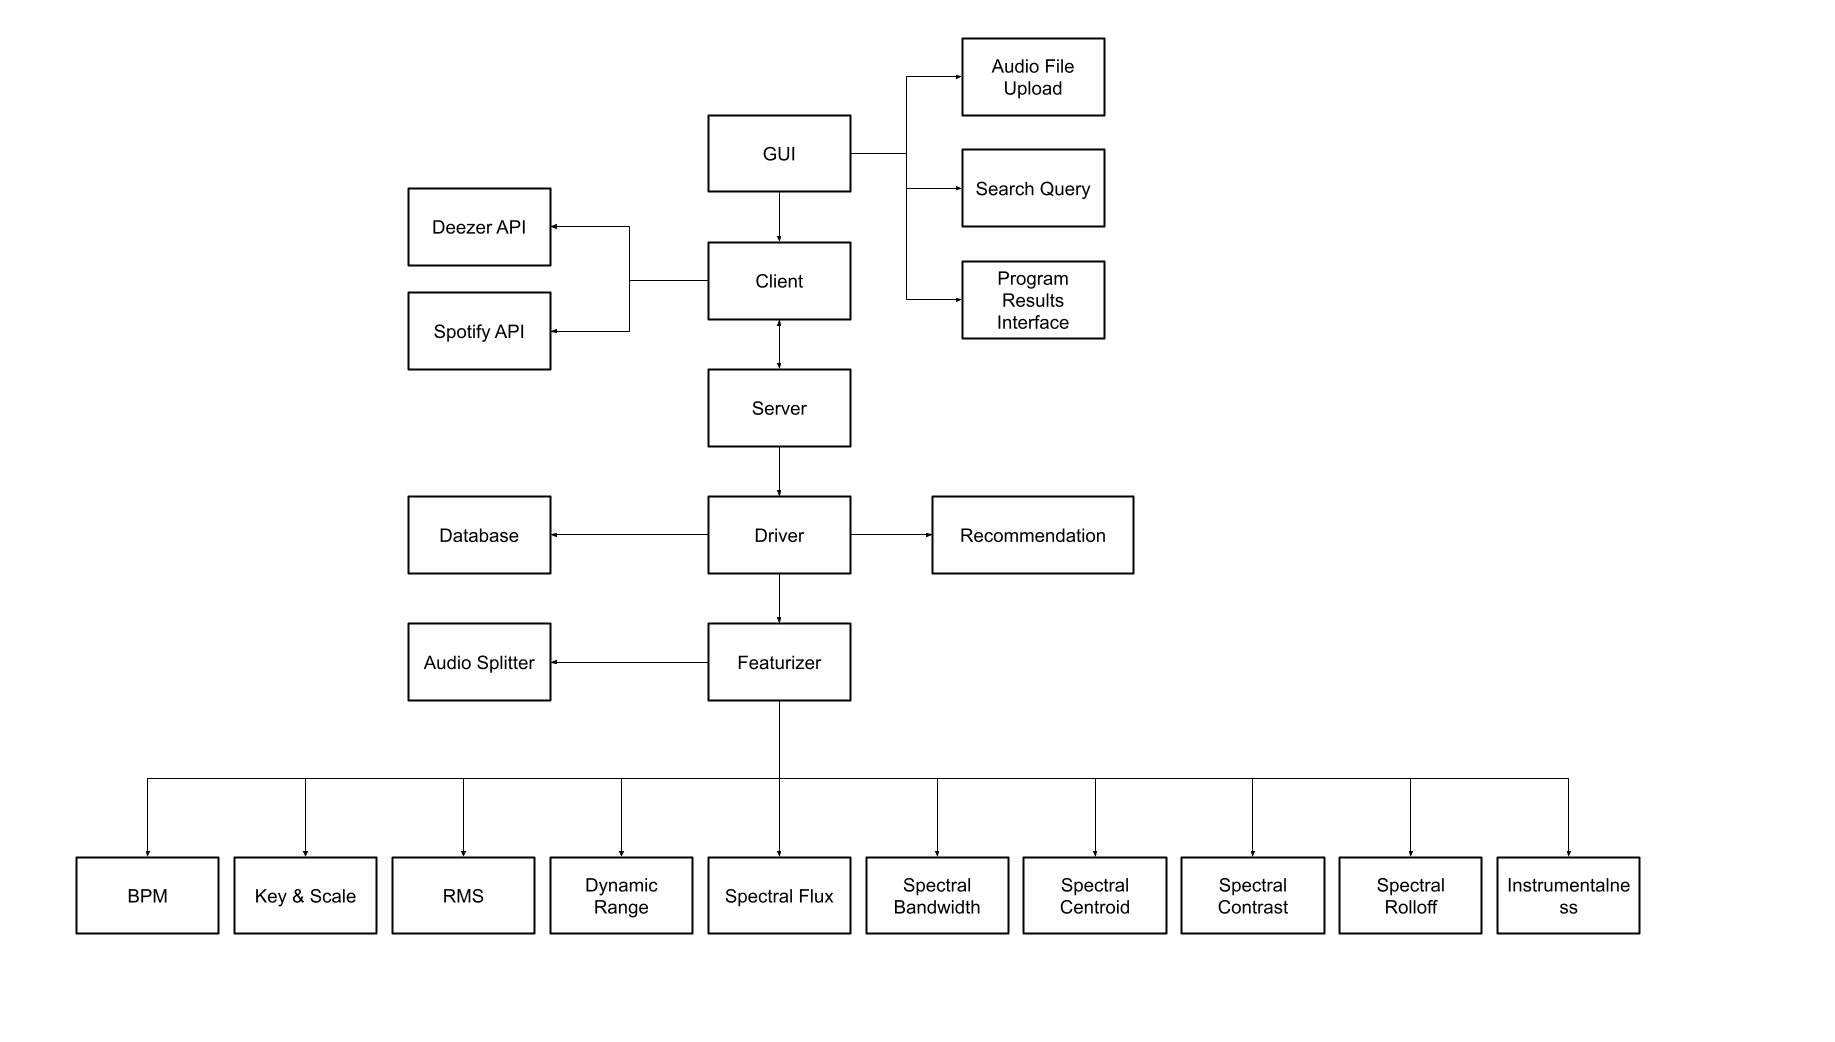
\includegraphics[width=0.7\textwidth]{UsesHierarchy.png}
\caption{Use hierarchy among modules}
\label{FigUH}
\end{figure}

%\section*{References}

\section{User Interfaces}


% Home Page Screenshot
\begin{figure}[h!]
    \centering
    
\includegraphics[width=0.8\textwidth]{UI_Images/Home_Page.png}
    \caption{Home Page - The initial screen where users start their interaction.}
    \label{fig:home_page}
\end{figure}

% Search Results Screenshot
\begin{figure}[h!]
    \centering
    
\includegraphics[width=0.8\textwidth]{UI_Images/Search_Results.png}
    \caption{Search Results - Shows the top matches for a user’s search query.}
    \label{fig:search_results}
\end{figure}

% Select Genre Screenshot
\begin{figure}[h!]
    \centering
    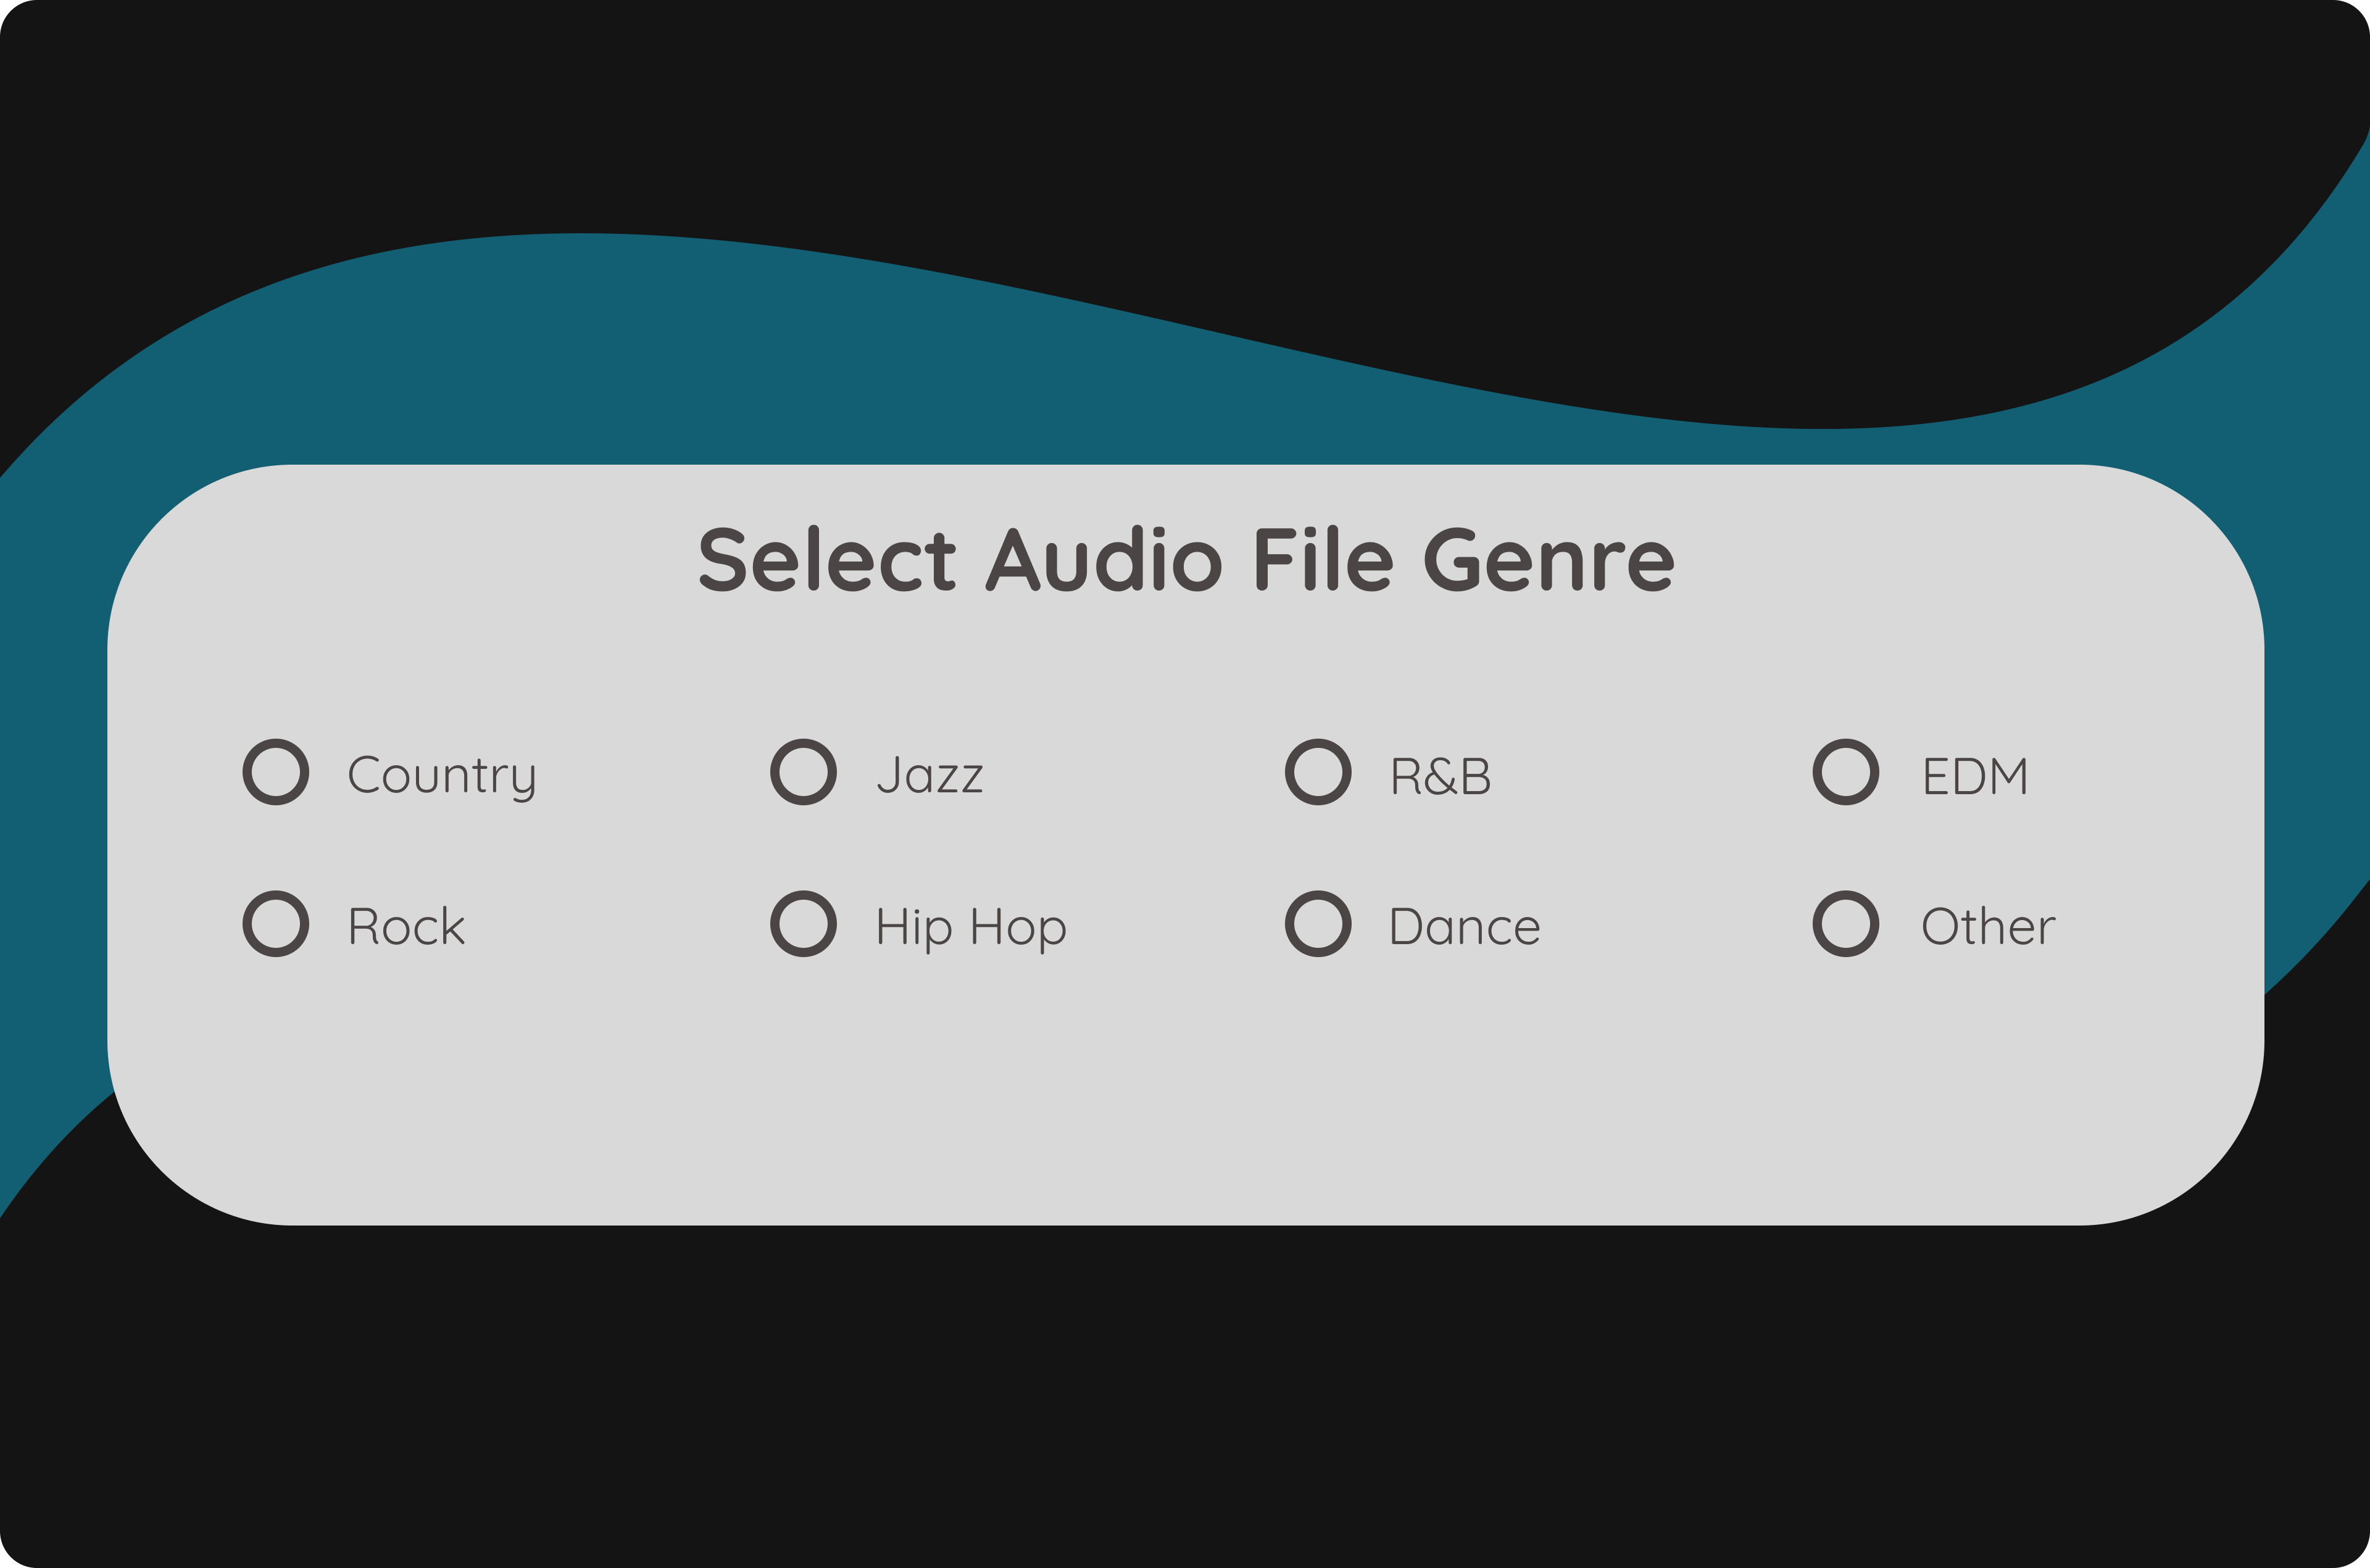
\includegraphics[width=0.8\textwidth]{UI_Images/Select_Genre.png}
    \caption{Select Genre - Allows users to specify the genre for uploaded audio files.}
    \label{fig:select_genre}
\end{figure}

% Loading Page Screenshot
\begin{figure}[h!]
  \centering
  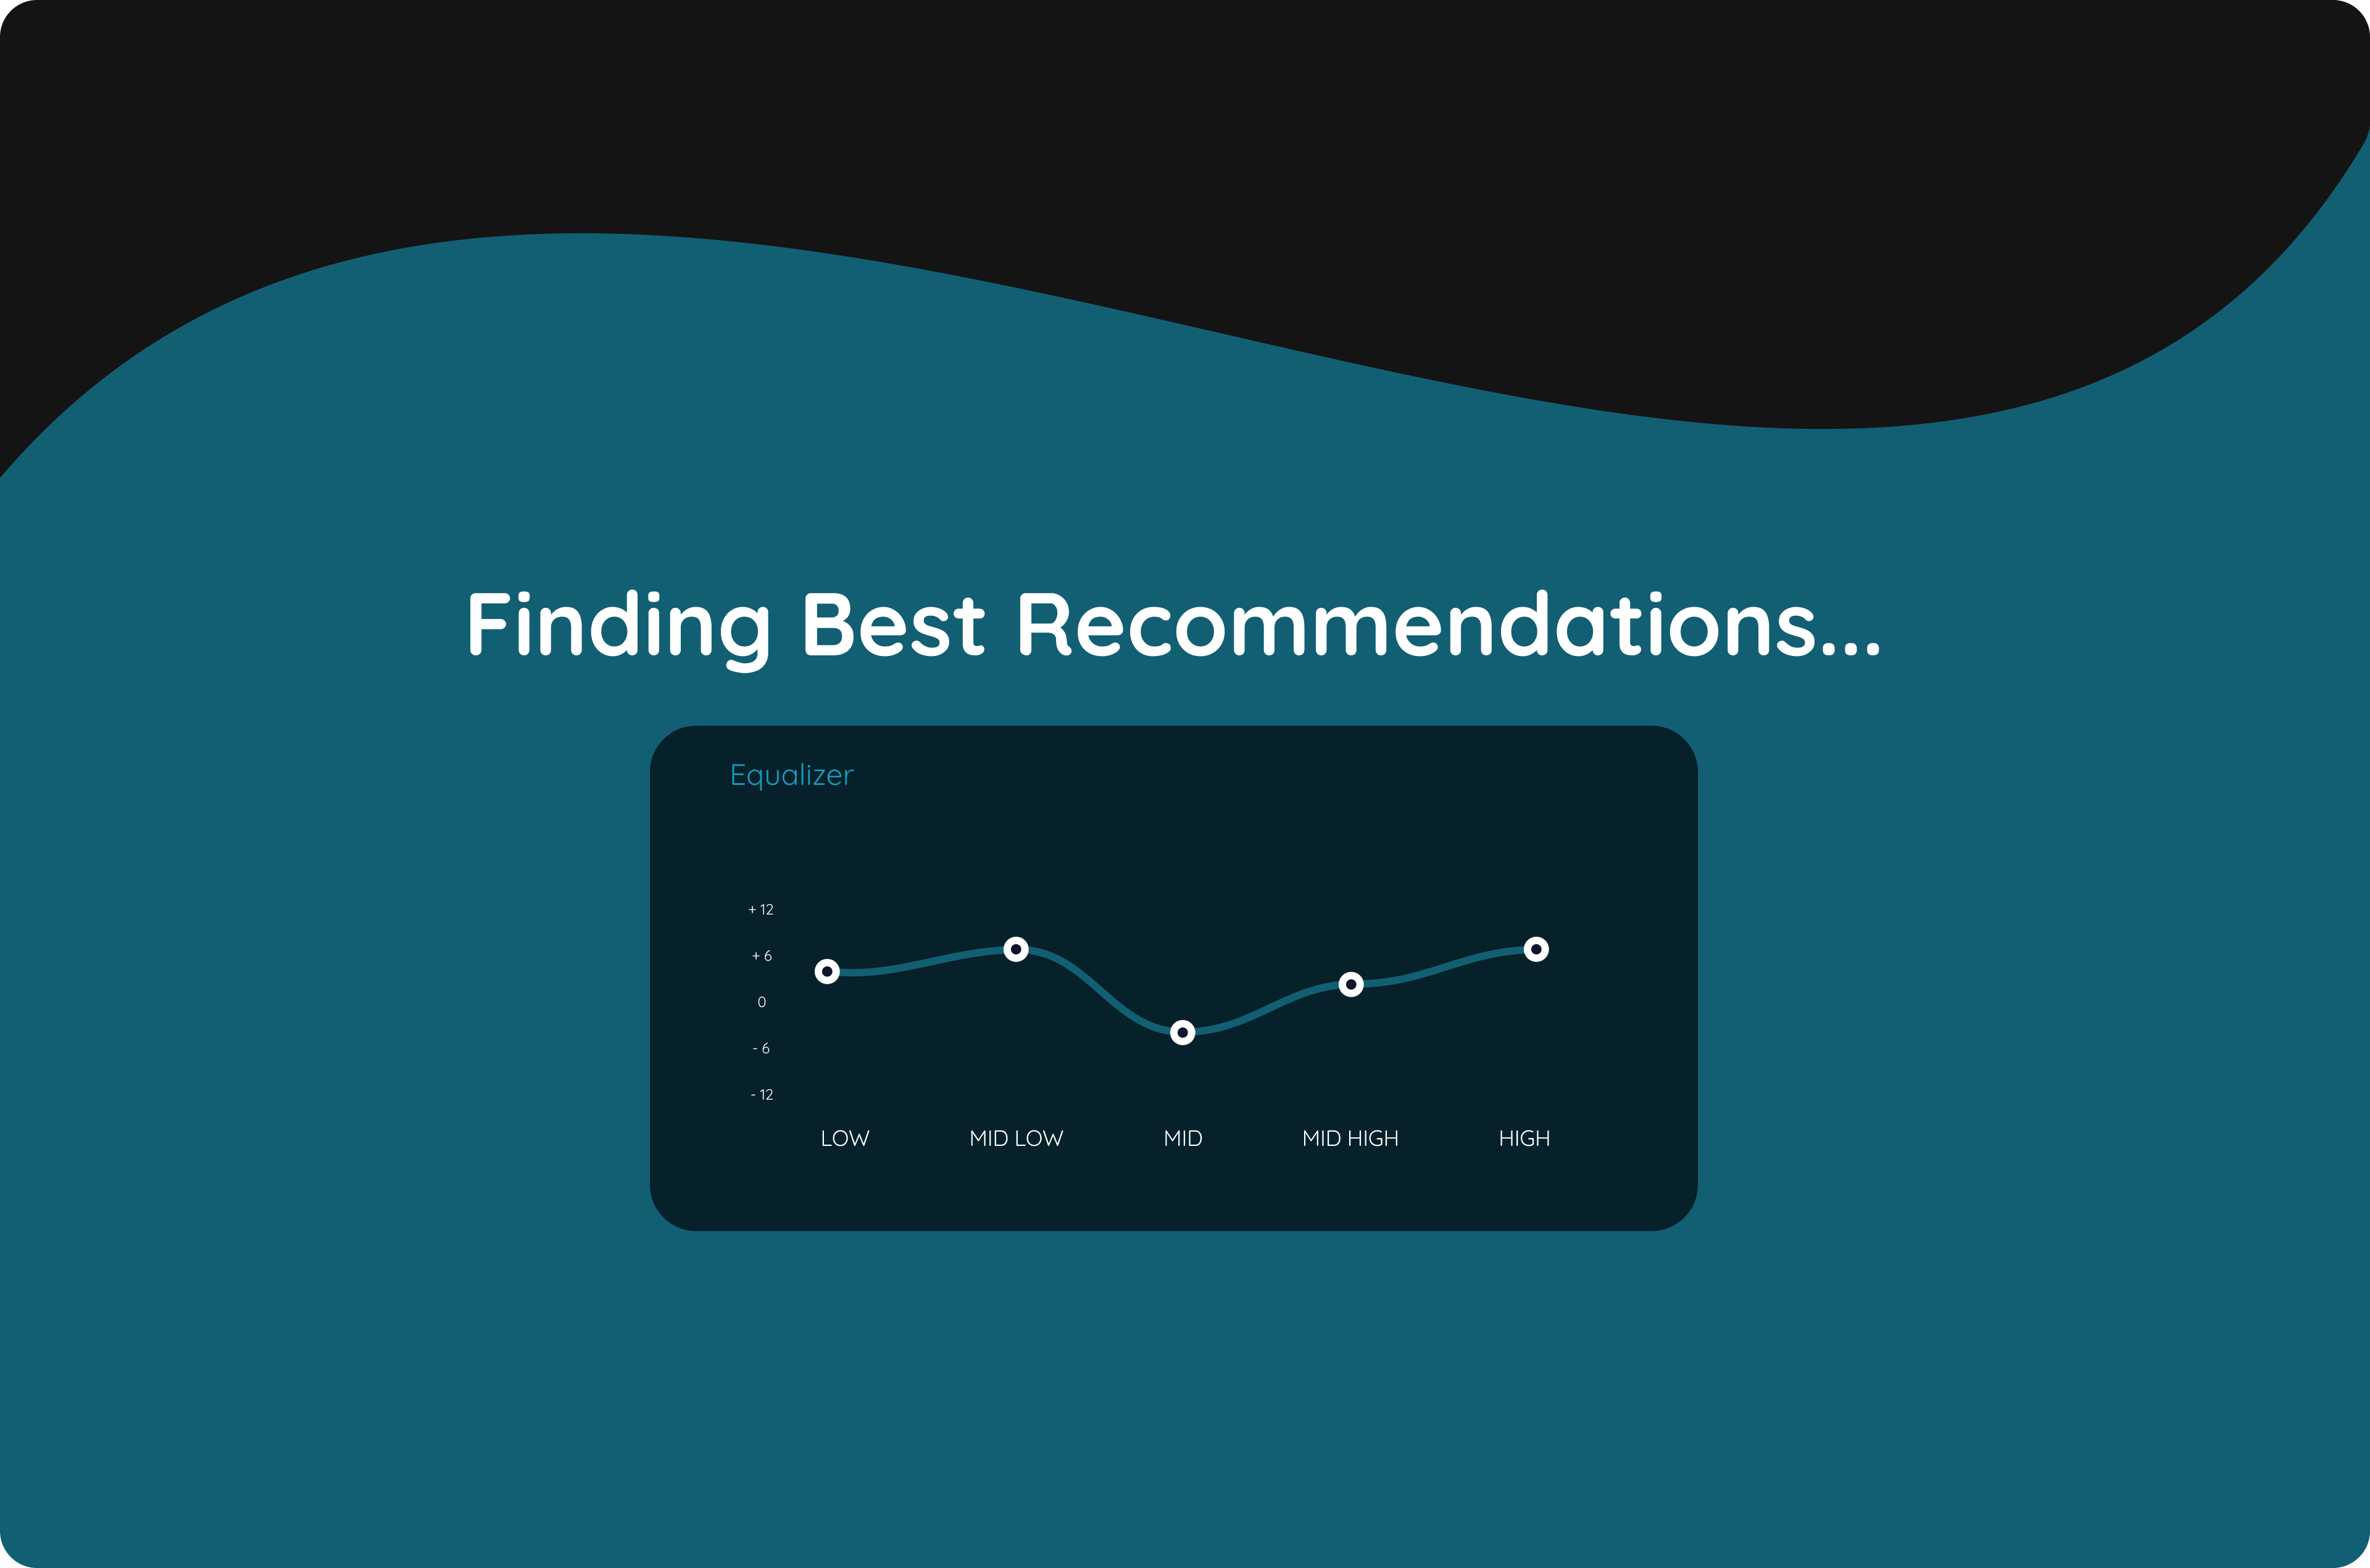
\includegraphics[width=0.8\textwidth]{UI_Images/Loading_Page.png}
  \caption{Loading Page - Indicates that the application is processing a request.}
  \label{fig:loading_page}
\end{figure}

% Results Page Screenshot
\begin{figure}[h!]
  \centering
  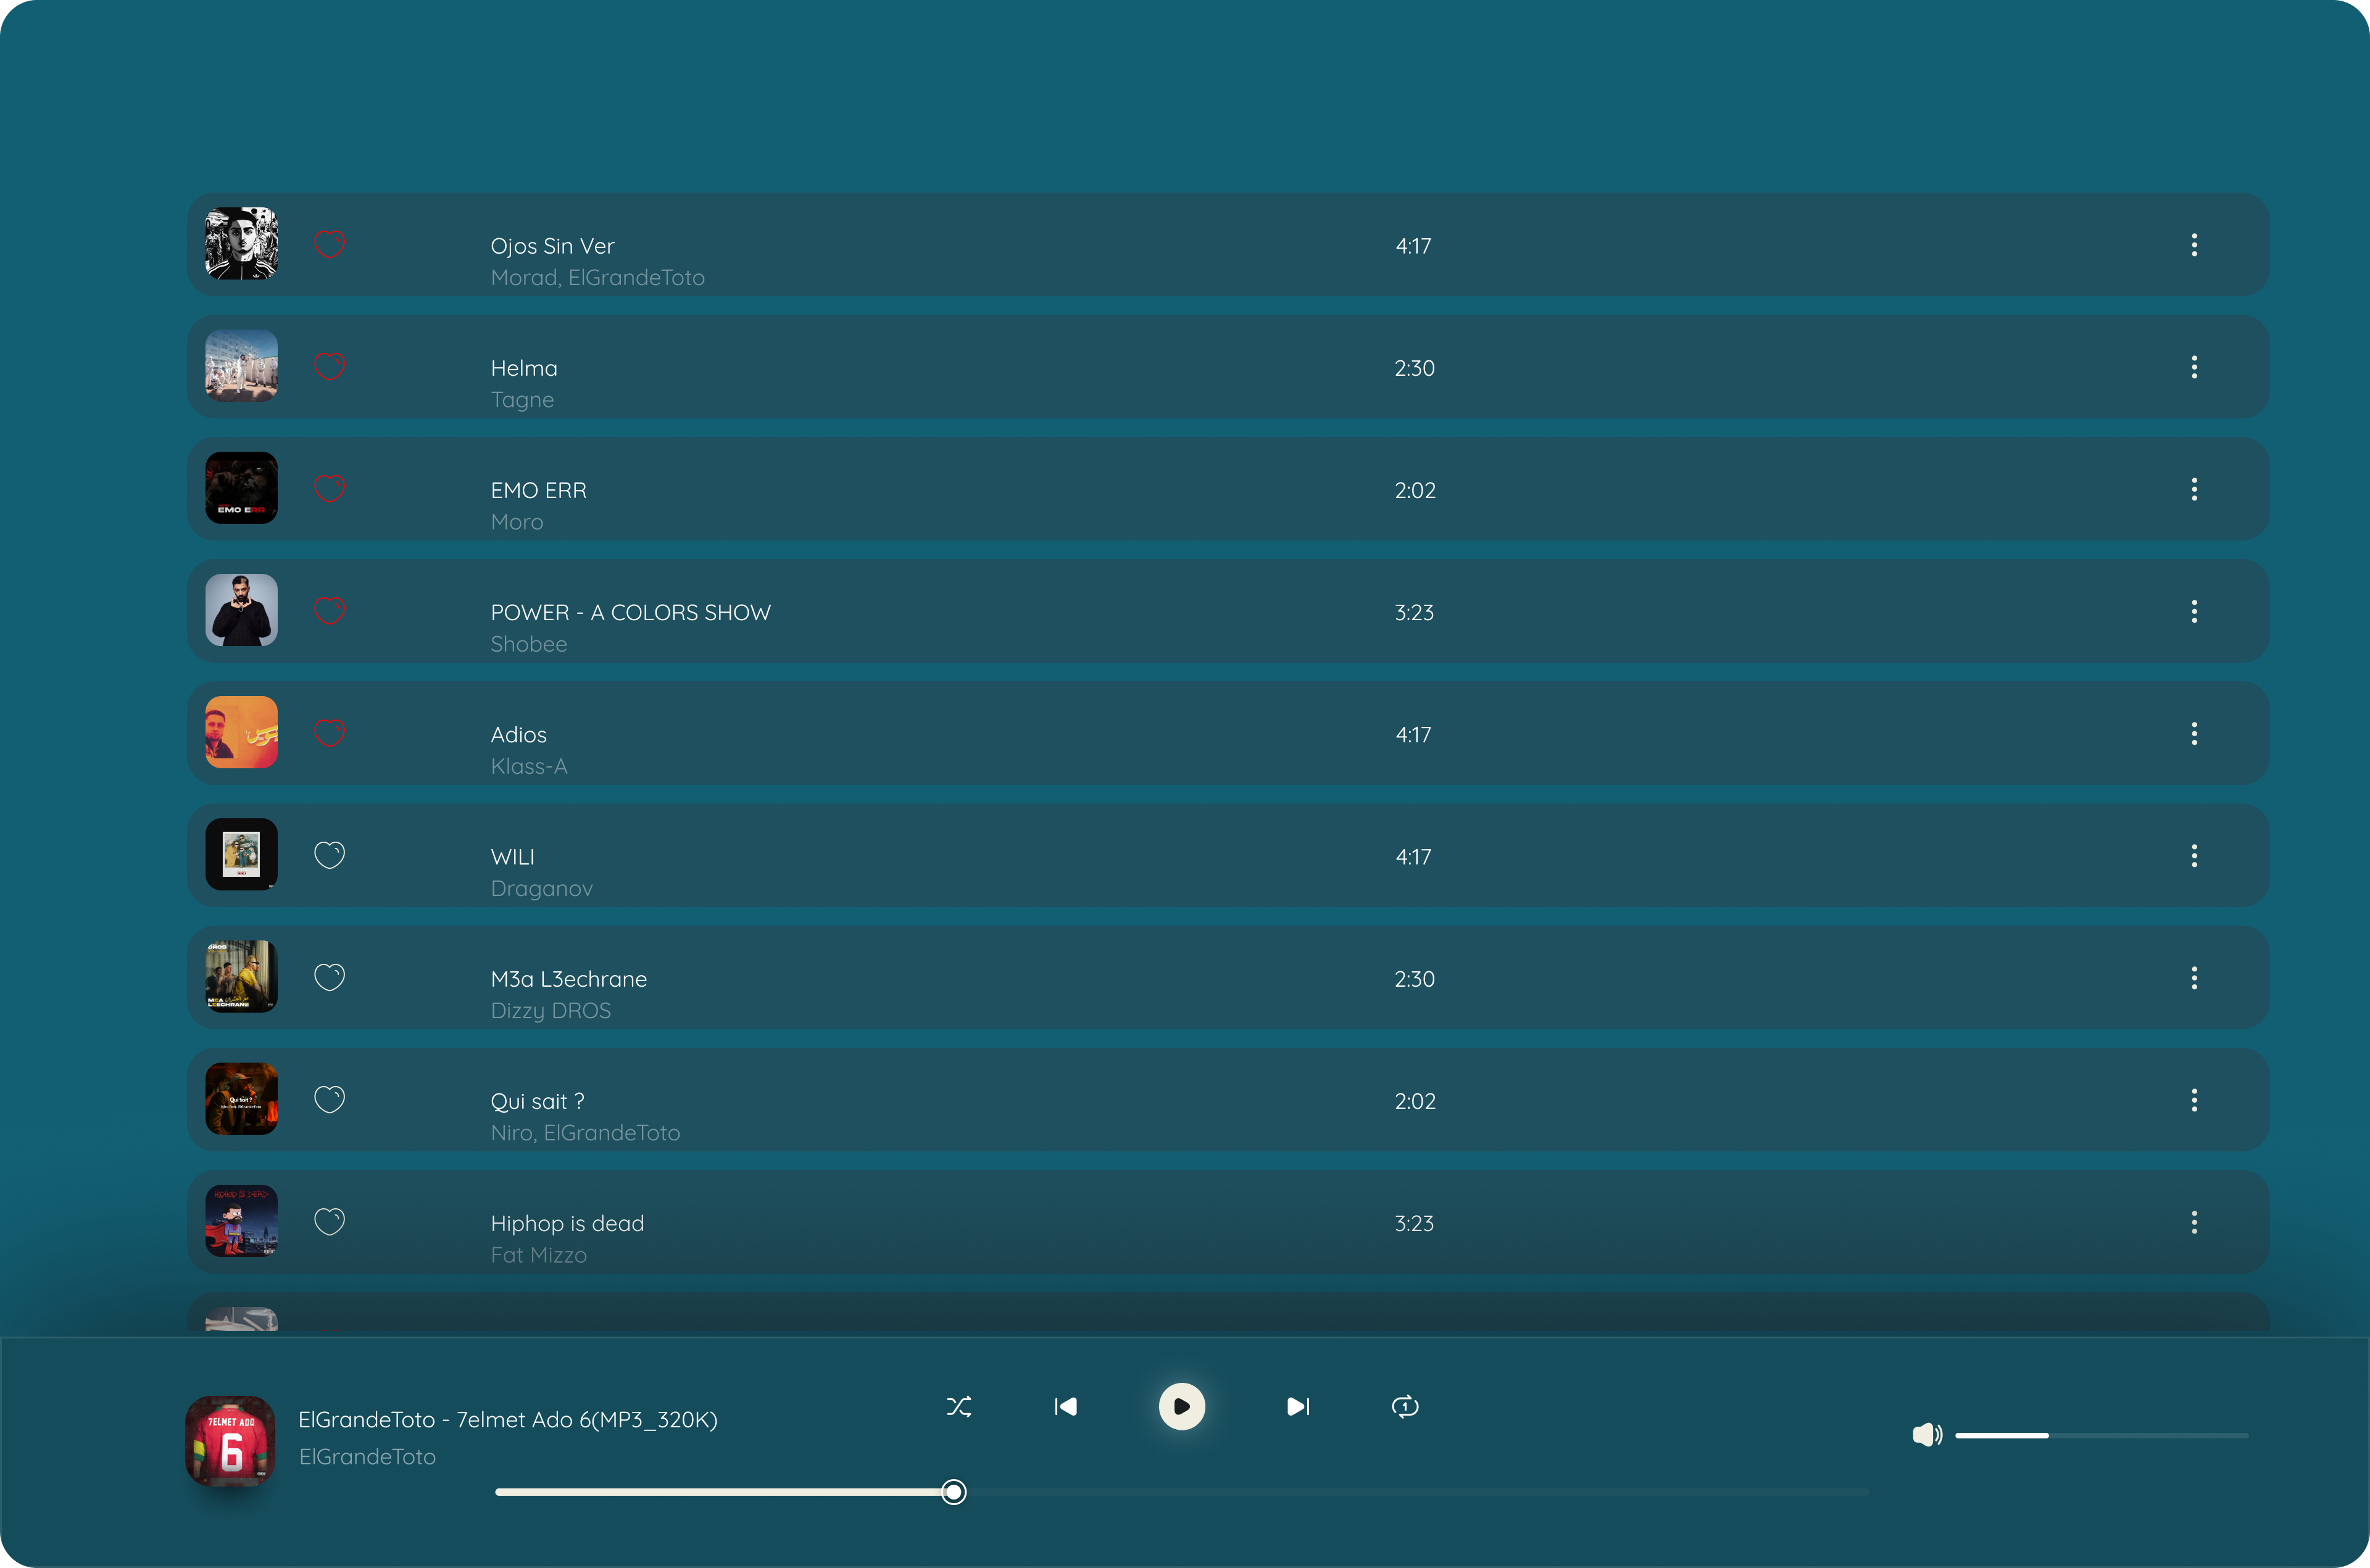
\includegraphics[width=0.8\textwidth]{UI_Images/Results_Page.png}
  \caption{Results Page - Displays the recommendation results.}
  \label{fig:results_page}
\end{figure}


%\wss{Design of user interface for software and hardware.  Attach an appendix if needed. Drawings, Sketches, Figma}
\section{Design of Communication Protocols}
Our design features 2 modules that have to do communication. They are listed as such: 
\begin{itemize}
  \item Client communication module
  \item Server communication module
\end{itemize}
The communication between the frontend systems is done simply through funtion calls. In order to send data (input type, audio data, song ID) from the frontend the user 
interacts with to the backend (the server) this will be done through encrypted data sent to the hosted server. This would be done by using
a RESTFUL interface as this is currently the most common method. Using standard REST API, the payload passed is a regular JSON object with 
a label for search or file input (the type of input) as that changes the behavior of the backend and the actual song ID itself. 

\section{Timeline}

The following timeline outlines the key milestones and activities planned for the development and refinement process:

\begin{itemize}
    \item \textbf{January 6th - January 17th:} Finalize the design document, decide on features and finalize on software architecture.
    \item \textbf{January 18th - January 20th:} Focus on refining the SRS, Hazard Analysis, and VnV documents.
    \item \textbf{January 20th - January 21st:} Conduct a meeting with Dr. MvM with a well-defined agenda to review progress and receive feedback.
    \item \textbf{January 22nd - January 23rd:} Engage with user groups to gather additional insights and validate design decisions.
    \item \textbf{January 23rd onwards:} Begin work on Rev 0 of the project deliverables, incorporating feedback from user groups and the advisor meeting.
    \item \textcolor{red}{\textbf{Feb 4th:} Revision 0 demo: Demonstration of the completed project.}
    \item \textcolor{red}{\textbf{March 10th:} VnV Report: Completed testing of the project.}
    \item \textcolor{red}{\textbf{March 27th:} Supervisor Final Demonstration.}
    \item \textcolor{red}{\textbf{April 8th:} Rev1: Final Documentation Completion}
    \item \textcolor{red}{\textbf{April 8th:} Capstone Expo}
\end{itemize}

All team members are responsible for the tasks described in this timeline breakdown are features in the
\hyperlink{https://github.com/AhmedAl-Hayali/GenreGuru/issues/278}{Post-Winter break Check-in} Issue.



%\wss{Schedule of tasks and who is responsible}

%\wss{You can point to GitHub if this information is included there}

\bibliographystyle {plainnat}
\bibliography{../../../refs/References}

\newpage{}

\end{document}